% THIS IS AN EXAMPLE DOCUMENT FOR VLDB 2012
% based on ACM SIGPROC-SP.TEX VERSION 2.7
% Modified by  Gerald Weber <gerald@cs.auckland.ac.nz>
% Removed the requirement to include *bbl file in here. (AhmetSacan, Sep2012)
% Fixed the equation on page 3 to prevent line overflow. (AhmetSacan, Sep2012)
\documentclass{vldb}

\usepackage{subfigure}
\usepackage{color}
\usepackage{balance}  % for  \balance command ON LAST PAGE 
\usepackage{graphicx}
\usepackage{epstopdf}  % used for generating pdf 
\usepackage[english]{babel}
\usepackage{amsmath}
\usepackage{graphicx}
\usepackage{caption}
\usepackage[compress]{cite}
\usepackage{amsfonts} 

% \let\proof\relax
% \let\endproof\relax
\usepackage{amsthm}


\usepackage{caption}
\usepackage{color}
\usepackage[ruled]{algorithm}
\usepackage{algorithmic}
\renewcommand{\algorithmiccomment}[1]{\bgroup #1 \egroup}




\newcommand{\ie}[0]{\textit{i.e.}}
\newcommand{\eg}[0]{\textit{e.g.}}
\newcommand{\etal}[0]{\textit{et al.}}
\newcommand{\wrt}[0]{\textit{w.r.t.}}


\newcommand{\keobf}{\textit{$(k,\epsilon)$-obf}}
\newcommand{\argmin}{\operatornamewithlimits{argmin}}
\newcommand{\genobf}{\texttt{\textbf{genObf}}}
\newcommand{\ere}{$\mathcal{E}RR-$eval}
\newcommand{\pg}{\mathcal{G}}
\newcommand{\Constraint}{$\mathcal{C}$}
\newcommand{\Number}{\|v\|}


\theoremstyle{plain}
\newtheorem{definition}{Definition}
\newtheorem{problem}{Problem}
\newtheorem{example}{Example}
\newtheorem{observation}{Observation}
\newtheorem{lemma}{Lemma}

\newcommand{\methodName}{Squid}
\newcommand{\capMethodName}{SQUID}
\newcommand{\soaName}{Obf}

\begin{document}


% ****************** TITLE ****************************************

\title{Sharing Uncertain Graphs with Syntactic Anonymity}
%\subtitle{[Extended Abstract]
%\titlenote{A full version of this paper is available as\textit{Author's Guide to Preparing ACM SIG Proceedings Using \LaTeX$2_\epsilon$\ and BibTeX} at \texttt{www.acm.org/eaddress.htm}}}


\numberofauthors{3} 

\author{
       \alignauthor
       Dongqing Xiao\\
              \affaddr{Worcester Polytechnic Institute}\\
              \affaddr{100 Institute Road}\\
              \affaddr{Worcester, MA, USA}\\
              \email{dxiao@wpi.edu}
       % 2nd. author
       \alignauthor
       Mohamed Elatbakh \\
              \affaddr{Worcester Polytechnic Institute}\\
              \affaddr{100 Institute Road}\\
              \affaddr{Worcester, MA, USA}\\
              \email{@wpi.edu}
       % 3rd. author
       \alignauthor 
       Xiangnan Kong \\
              \affaddr{Worcester Polytechnic Institute}\\
              \affaddr{100 Institute Road}\\
              \affaddr{Worcester, MA, USA}\\
              \email{xkong@wpi.edu}
}

\maketitle

\begin{abstract}
Many graphs in real-world applications, such as social network and business to business network, are not deterministic but are uncertain. Related research such as social science and viral marketing requires open access to such uncertain graph datasets. While sharing these datasets often risks exposing sensitive data to the public. Current works mainly concern about privacy issues with deterministic graph sharing. 
The uncertain scenario is overlooked.

In this paper, we study the problem of sharing uncertain graphs with syntactic anonymity. 
We first show conventional methods are not applicable for sharing uncertain graph. 
By disregarding the possible world semantic of uncertain graphs, they significantly disrupt the stochastic structure. Our work seeks a solution to share meaningful probabilistic graphs without compromising user privacy. We develop a syntactically private algorithm, Squid, for solving this problem. It integrates the possible world semantic into the core of anonymization. It enables a fine-grained, uncertainty-aware control over the injected noise. We apply our method to real uncertain graphs and show its efficiency and practical utility. 
\end{abstract}
\section{Introduction}

\label{sec:Intro}

% Graph-- Uncertain Graph--Examples 
Graphs are widely used to capture the relationships in emerging applications, such as business to business (B2B) and social networks. 
Sometimes, the existence of the relationship between two entities is uncertain (probabilistic). For instance, in social networks, nodes represent individual users, while edges represent friendship or trust link among them.  Usually, the link strength is derived by inference and prediction models built on interaction details~\cite{Adar_Managing_2007,Kempe_Maximizing_2003}. While edge probability denotes the accuracy of a link prediction or the trust of one person on another. 
In these applications, the data can be modeled and shared as uncertain graphs whose edges carries a probability of existence. The probability represents the confidence that the relationship holds in reality. 

\begin{figure}[!htb]
    \subfigure[Social Trust Network]{\label{fig:socialNetwork}
      \begin{minipage}[l]{0.45\columnwidth}
        \centering
        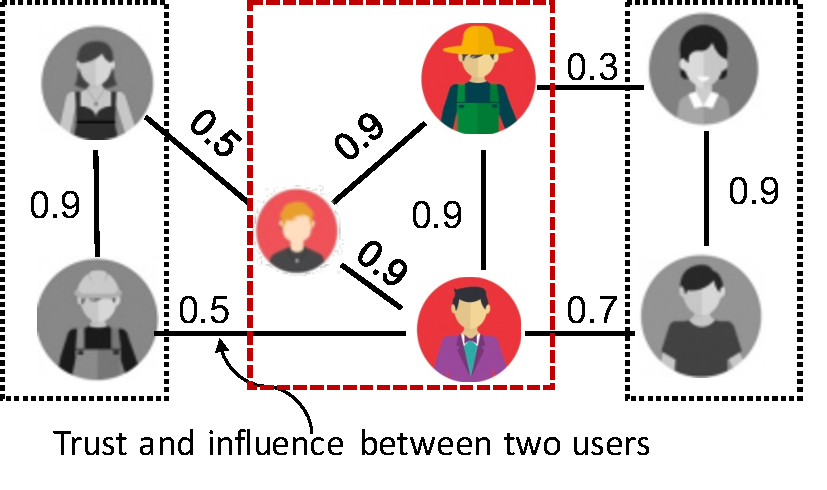
\includegraphics[height=2.3cm]{ill/SocialNetwork.pdf}
      \end{minipage}
      }
    \subfigure[B2B Network]{\label{fig:b2bNetwork}
      \begin{minipage}[l]{0.45\columnwidth}
        \centering
        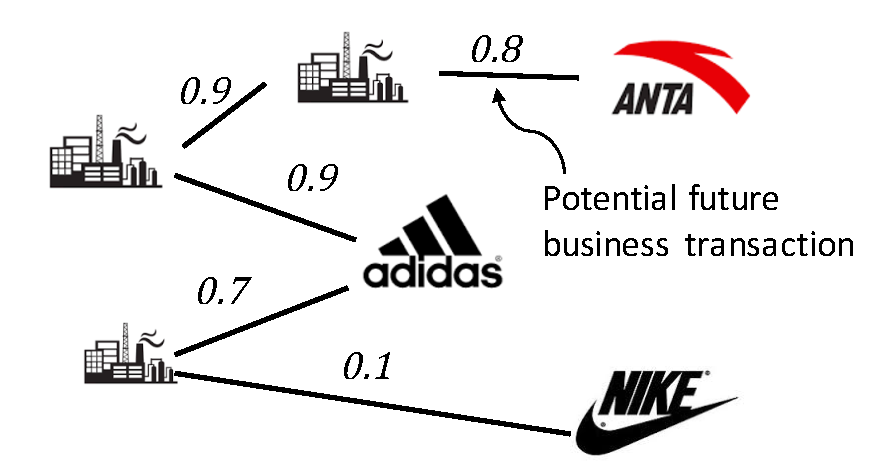
\includegraphics[height=2.3cm]{ill/B2BNetwork.pdf}
      \end{minipage}
      }
    \vspace{-6pt}
    \caption{Real-world uncertain graphs with privacy concerns.}
    \label{fig:motivation}
    \vspace{-10pt}
\end{figure} 

% Sharing--Privacy--Examples 
These uncertain graphs are invaluable for scientific research and commercial applications e.g., understanding social interactions, information propagation and advertising~\cite{Kempe_Maximizing_2003,Cho_Friendship_2011}. 
Compared to sharing the results of graph mining, graph sharing gives greater flexibility as recipients can perform unlimited analysis, data explosion with novel methods.

However, sharing these uncertain graphs could seriously jeopardize the privacy of users or entities profiled inside.
In social trust network, the trust relationships among users, which significantly impact users' behaviors, are usually probabilistic.  They are useful in social interaction study and micro-targeting~\cite{Kempe_Maximizing_2003}. However, users are unwilling to share such confidential information with potential adversaries. In B2B networks, business operators also hesitate to share transaction patterns as it relates to confidential business models. Such tension is raising the question of sharing uncertain graphs without compromising privacy. 

% State-of-Art %
A number of privacy preserving graph sharing schemes have been studied in the deterministic scenario~\cite{Liu_Towards_2008,Ying_Randomizing_2008,Wang2011,Liu_Privacy_2009,Nguyen_Anonymizing_2015,Sala_Sharing_2011,Xiao_Differentially_2014,lee2011}, though many problems still remain unexplored in the uncertain scenario.
\begin{figure}[!htb]
  \centering
  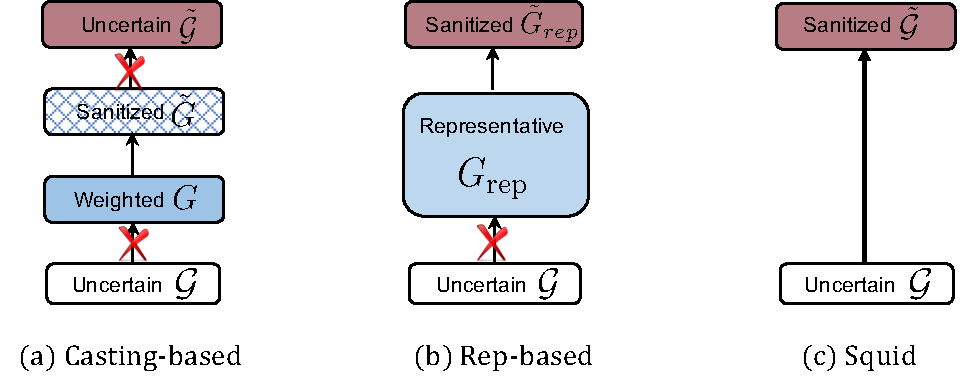
\includegraphics[width=0.9\linewidth]{ill/methods.pdf}
  \caption{Illustration of three anonymization approaches.}
\end{figure}

An obvious approach is to convert the uncertain graph sharing problem into the deterministic one by casting edge probabilities as edge weights. 
While, the general idea is appealing, the casting-based method is inadequate to provide desirable utility for uncertain graph. 
By disregarding the possible world semantics of the uncertain graph, casting-based approach, as later illustrated, fails to reflect uncertain graph properties such as connectivity, dense subgraphs correctly~\cite{Zhao_Detecting_2014,Hua_Probabilistic_2010}. 
Hence, the casting-based scheme could produce poor results in the uncertain scenario even if the weighted graph anonymization algorithm is good. 

\textbf{Example}. \emph{Connectivity of deterministic subgraphs is generally measured by the concept of cut, which is defined as the sum of weights of intra edges. Generally, the bigger the cut, the harder to separate two subgraphs. In Figure~\ref{fig:motivation}(a), the equal cut $C(SG_{1},SG_{2})=C(SG_{3},SG_{2})=1$ implies the identical connectivity of $SG_{1}$ and $SG_{3}$ {\wrt} $SG_{2}$. However, with the possible world semantics, we know the probability to separate $SG_{1}$ and $SG_{2}$ is $(1-0.5)^{2}=0.25$, and that to separate $SG_{2}$ and $SG_{3}$ is $(1-0.3)(1-0.7)=0.21$. Hence, in fact, $SG_{2}$ is closer to $SG_{1}$ than to $SG_{3}$. }

In the previous work~\cite{Xiao:2018}, we ever proposed a representative-based method, based on the idea of processing uncertain graph through representative instances~\cite{Parchas_Gullo_Papadias_Bonchi_2014}.
It first extracts a single deterministic representative instance $G$ that capture structural properties of the uncertain graph.
After that, anonymization can then proceed efficiently on $G$ using conventional algorithms, regardless of the uncertainty.  
The advantage of this method is that it does not require new anonymization techniques. 
However, the representative-based method is not always feasible. 
The detachment of edge uncertainty deteriorates the data utility. 

As ever discussed, conventional graph anonymization schemes are inadequate to share uncertain graphs with a desirable trade-off between privacy and utility. 
It is worthwhile to consider developing the specially optimized solution for handling following challenges. 

$\bullet$~\textup{\emph{Stochastic Privacy Attacks.}}~~Edge uncertainty plays an indispensable role in the uncertain graph model. Discarding them in the release is impractical.  
However, the extra release of edge uncertainty makes privacy protection far more difficult as it empowers the adversary and makes the profiled entity more vulnerable. 
To this end, we clarify the potential re-identification attack and adopt a privacy notion for releasing privacy-preserving uncertain graphs.

$\bullet$~\textup{\emph{Stochastic Utility Loss Metric.}}~~It is challenging to maintain the structure when the uncertain graph is modified to pursue anonymity. 
The structural distortion incurred is evaluated by the specially designed utility loss metric.  
It aims to safeguard the utility of the release graphs.  
Unfortunately, current graph utility loss metrics such as graph edit distance~\cite{Liu_Towards_2008}, spectrum discrepancy~\cite{Ying_Randomizing_2008}, community reconstruction error~\cite{Wang2011} and shortest path discrepancy~\cite{Liu_Privacy_2009} 
are not suitable in our problem setting because of the ignorance of edge uncertainty.
In this context, the discrepancy w.r.t the uncertain graph reliability becomes a useful criterion. It evaluates the connectivity difference in the context of the entire graph and meanwhile utilizes the possible world semantics. 

$\bullet$~\textup{\emph{Intractable Search Space.}}~~Informally, our goal is to find a sanitized graph with the desired level of privacy with as few graph mutations as possible. 
Even the simple deterministic graph anonymization problem, {\ie}, is known to be NP-hard when mutations are limited to edge additions and deletions~\cite{Hartung_Theory_2015}. 
In the probabilistic scenario, edge modifications are no longer limited to edge addition and deletion, but can be infinite probability deviations. 
Exhaustive search is computationally intractable if the number of edges is large. 
It makes the uncertain graph anonymization problem very challenging. 
In this work, we approximate the problem of interest via a randomized algorithm, which built on the basis of meta-heuristics. 

In this work, we propose a novel sanitization solution tailored towards uncertain graphs via incorporating possible world semantics and test it on three real-life network datasets. We analyze the utility of sanitized graphs (uncertain ones) in two scenarios: extracting statistics for graph analysis, and performing influence prorogation. We show our method preserves as much the stochastic nature of the original uncertain graph as possible while injecting necessary structural noise to guarantee a desirable level of privacy. We also show that significant improvement of our methods over casting-based and representative-based methods. 
Specifically, we make the following contributions.
\begin{itemize}
\item We are the first to formulate the uncertain graph sharing problem. 
 We show the potential re-identification attack and present a practical privacy notion. 
\item Motivated by the use of connectivity error, we propose a utility loss metric on the basis of reliability. It evaluates the connectivity difference in the context of the entire graph and also utilizes the possible world model. 
\item To alleviate the combinational intractability, we propose a randomized algorithm boosted by the hybrid of uncertainty-aware heuristics. It excels in identifying a population of sanitized results with good quality efficiently.
\item We conduct extensive experimental studies to demonstrate efficiency and practical utility of our algorithms. The results demonstrate a significant advantage over the conventional methods that do not directly consider edge uncertainties.
\end{itemize}

The rest of the paper is organized as follows. In Section~\ref{sec:relatedWork}, we summarize related works, point out the limitation of existing methods, and clarify our distinct privacy goal. In Section~\ref{sec:notation} we formulate the uncertain graph-anonymization problem. Sections~\ref{sec:soa} –~\ref{sec:method} present our anonymization approach for releasing privacy-preserving uncertain graph.  In Section~\ref{sec:ex} we apply our method to several real-world uncertain graphs and demonstrate its performance, practical utility and efficiency. 
\section{Related Work}
\label{sec:relatedWork}
A significant amount of prior work has been done on protecting the privacy of network datasets.
The comprehensive survey is out of the scope of this paper. 
Here, we briefly summarize related work and clarify our privacy goal. 

\textbf{Syntactic Privacy.}~~
Early works on privacy-preserving network releasing focus on developing anonymization techniques.
Many of them modify the graph structure in subtle ways that guarantee privacy but keep much of graph structure for release. 
The released graph is available for all the analysis tasks. 
These approaches usually provide privacy protection against specific de-anonymization attacks. 
Most of them employ syntactic privacy models derived from $k$-anonymity~\cite{Sweeney:2002:KAM:774544.774552} which requires creating $k$ same entities ({\eg} neighborhoods, degree nodes) to blend victims. 

Related anonymization methods can be classified into four main categories: (1) Clustering-based generalization~\cite{Hay_Anonymizing_2007,Bhagat_Class_2009,hay2010resisting}; (2)~{\em Edge modification}~\cite{Liu_Towards_2008, Zhou_Preserving_2008, Zou:2009, Wang2011, Wu_k_2010, Skarkala_Privacy_2012}; 
(3)~{\em Edge randomization}~\cite{Liu_Privacy_2009,Ying_Randomizing_2008, Ninggal_Utility_2015};
and~(4)~{\em Uncertainty semantic-based modifications} which add uncertainty to some edges and thus converting the deterministic graph to an uncertain version for anonymity~\cite{Boldi_Injecting_2012, Nguyen_Anonymizing_2015}. 

In the first category, Hay {\etal}~\cite{Hay_Anonymizing_2007} proposed to generalize a network by clustering nodes and only publish the hyper-graph ($\#$ of nodes in each partition with $\#$ of edges within and across partitions). Campan {\etal}~\cite{Campan2008} studied the attributed graph case with a similar solution. 
Cohen {\etal}~\cite{Cohen2013} presented a sequential clustering algorithm with better utility preserving. While, Cormode{\etal} \cite{Bhagat_Class_2009} payed attention to attributed-based matching attack. To this end, their method marks the mapping by clustering the nodes and corresponding real world entities into groups. 

In the second category, Liu {\etal}~\cite{Liu_Towards_2008} focused on resisting degree-based entity re-identification attacks. They propose to add and delete edges to pursue $k$-degree anonymity. Zhou {\etal}~\cite{Zhou_Preserving_2008} consider stronger re-identification attack based on radius-one subgraph. Zhou~{\etal}~\cite{Zou:2009} assume that the adversary knows the compute graph. Their algorithms use edge addition and deletion to make graph $k$-Automorphism.  

In the third category, Hay {\etal} \cite{Liu_Privacy_2009} study the use of random perturbation for identity obfuscation. They consider the basic degree-based re-identification of nodes. Besides, they propose to quantify the level of anonymity that is provided for the given node $v$ in the real network by the perturbed graph as the inverse of the maximum of the belief probability $Pr(v|u)$. Ying {\etal} \cite{Ying_Randomizing_2008} compare random perturbation methods to the method of $k-$degree anonymity. Their experiments over two datasets (Enron and Pollblogs) show the deterministic edge modification methods for $k$-degree anonymity preserve the graph structure better than random perturbation methods.

The uncertainty semantic-based approaches are known as the state-of-art ones because of their excellent privacy-utility trade-off, brought by the fine-grained perturbation leveraging the uncertain semantics. 
% add two-sentences about the works 
Our method belongs to the fourth category while for the probabilistic context. 

 
\textbf{Differential Privacy.}~~
The dependence of adversary knowledge makes graph anonymization methods are vulnerable to attackers with strong background knowledge than assumed. Such fact has similuated the use of differential privacy for more rigorous privacy guarntess. 
The recent research on applying differential privacy to graph data roughly falls into two directions. The first direction aims to release specific differentially private mining results, such as degree distributions, sub-graph counts, and frequent graph patterns~\cite{Xiao_Differentially_2014,Day:2016}. These methods only publish query result. However, there are many situations in which answering statistical queries simply does not achieve the purpose of sharing the graph.  
The second direction aims to share the meaningful graph. Most research in this direction~\cite{Sala_Sharing_2011,Proserpio_2012} projects an input graph to dK-series and ensures differential privacy on dK-series statistics. Later, private statistics are then either fed into generators or MCMC process to generate a fit synthetic graphs. While current techniques are still inadequate to provide desirable data utility for many graph mining tasks. Wang {\etal}~\cite{Wang_2013} propose to project a graph to the spectral domain and inject noise to the eigenvalues and eigenvector. This approch achieved significant improvement on efficiency, which, is still not able to achieve good data utility. Xiao {\etal}~\cite{Xiao_Differentially_2014} present a solution based on structural inference over the hierachical random graph model. This approach achieved the reasonable utility over real-life graph datasets. 

All the methods target at providing privacy guarantee to the deterministic graph. 
The uncertain scenario is unexplored. 

\subsection{Our Privacy Goal}
As ever discussed, existing methods fail to provide utility guarantee in the uncertain scenario. 
In this work, we try to move this line of research one step forward from the deterministic context to a broader probabilistic context. 
Our work seeks a solution to share meaningful uncertain graphs while preserving privacy.
We believe the anonymization process needed to be specially optimized to uncertain graphs.

There is a widespread belief that differential privacy and its offsprings are immune to various privacy attacks. It offers a guarantee bound $\epsilon$ on the loss of privacy due to the data release~\cite{Sala_Sharing_2011,Xiao_Differentially_2014}. However, there is no clear way to set general policy for choosing the privacy parameter $\epsilon$ for sufficient privacy guarantee~\cite{lee2011}. Its implications and impacts on the risk of disclosure in practice heavy depend on data detail. Thus, differential privacy is difficult to apply in practice. 

In contrast, the notion of syntactic privacy can be defined and understood based on the data schema. And, its parameters have a clear privacy meaning that can be understood independent of the actual data. Moreover, they have a clear relationship to the privacy regulation of individual identifiability (e.g., General Data Protection Regulation GDPR). 
Hence, we focus on sharing uncertain graphs with syntactic anonymity. 
\section{Problem Formulation}
\label{sec:notation}

In this section, we provide background on uncertain graphs, privacy attack and justify our choice of utility loss metric. 
On this basis, we present our formulation of the uncertain graph anonymization problem. 

\subsection{Uncertain Graph}
An uncertain graph $\mathcal{G}=(V,E,\mathit{p})$, is defined over a set of nodes $V$, a set of edges $E$, and a set of probabilities $\mathit{p}$ of edge existence. Following the literature~\cite{Potamias_K_2010,Zhao_Detecting_2014,Colbourn_Colbourn_1987}, we assume the possible-worlds semantics, and we consider the edge probabilities independent~\footnote{We leave the conditional probability model as a future
extension.}. An uncertain graph $\mathcal{G}=(V,E,\mathit{p})$ essentially represents a probability distribution over all of the certain graphs $G$ in the forms of which the uncertain graph may actually exist. 
The probability of observing any possible world $G_i=(V,E_{G_i})$ is    
\begin{equation*}
    Pr[G_i]=\prod_{e \in E_{G_i}} {\mathit{p}(e)} \prod_{e \in E \setminus E_{G_i}} 1-\mathit{p}(e)
\end{equation*}
\subsection{Privacy Attack}
\label{sec:AMPC}
\begin{figure}[!htb]
    \subfigure[Social Trust Network]{\label{fig:socialNetwork}
      \begin{minipage}[l]{0.46\columnwidth}
        \centering
        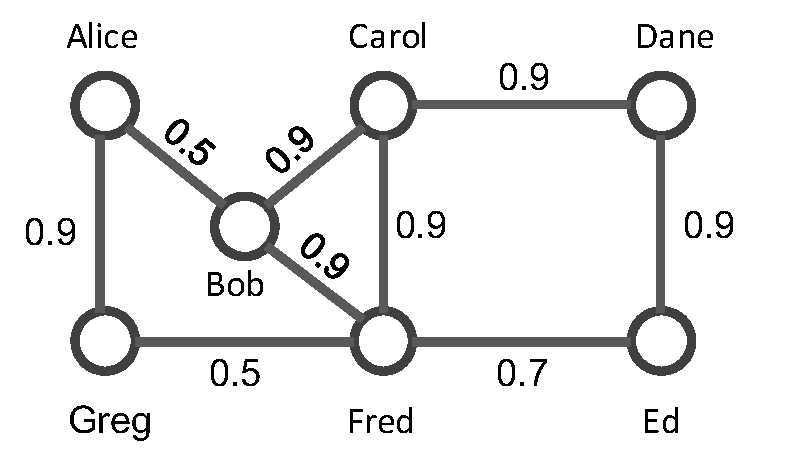
\includegraphics[height=2.7cm]{ill/example_source.pdf}
      \end{minipage}
      }
    \subfigure[The naive anonymization]{\label{fig:b2bNetwork}
      \begin{minipage}[l]{0.46\columnwidth}
        \centering
        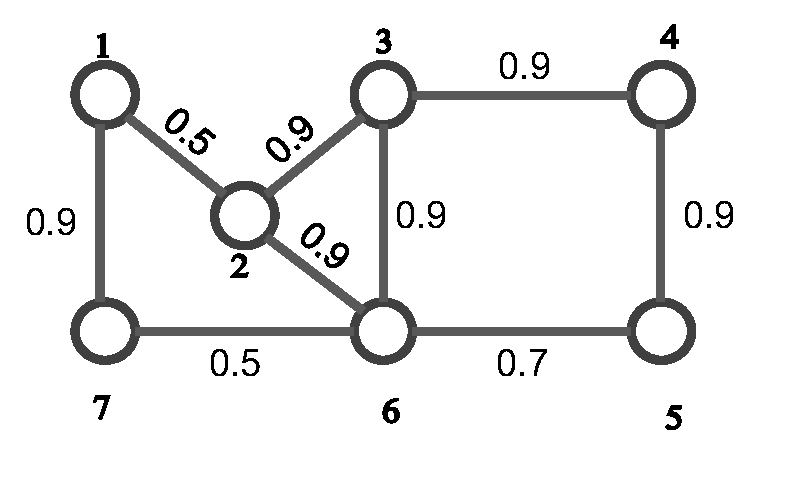
\includegraphics[height=2.7cm]{ill/example_output.pdf}
      \end{minipage}
      }
    \caption{The structural re-identification issue.}
    \label{fig:privacyAttack}
\end{figure} 
Apparently, simply removing the identities of the nodes before publishing the uncertain graph does not guarantee privacy.  The structure of the uncertain graph itself, and in its basic form the degree of the nodes, can be revealing the identities of individuals. 
In practice, the adversary may have access to external information about the entities in the graphs. This information may be obtained by the adversary's malicious actions. 
For example, for the uncertain graph in Figure~\ref{fig:privacyAttack}, the adversary might know that ``\emph{Fred has three or more \textbf{trust} neighbors}''. Such information allows the adversary to narrow down the set of candidates in the sanitized graphs.  The statement partially re-identify Fred as $\lbrace 2,3,6 \rbrace$ with \textbf{probabilities} respectively. 
Different to the deterministic scenario, posterior probabilities significantly vary over candidate nodes $\lbrace 2,3,6 \rbrace$ where $P(6|\text{Fred}) \simeq P(3|\text{Fred}) \gg P(2|\text{Fred})$.

As ever illustrated, nodes in uncertain graphs are vulnerable to the re-identification risk. Such Entity Re-identification (ER) can lead to additional disclosures. In this work, we focus on the ER attack as it is one of the most serious privacy problems. 
\subsection{Privacy Notion}
\label{sec:privacyNotion}
To resist ER attacks, we adopt $(k,\epsilon)$-obf, a variant of the well-known $k-$anonymity. It was proposed by Boldi {\etal} in ~\cite{Boldi_Injecting_2012}, where $k \ge 1$ is a desired level of obfuscation and $\epsilon \ge 0$ is a tolerance parameter. 

\textsc{Obfuscation Parameter}~~Similar to $k-$anonymity, $k-$obf requires blending every entity with other fuzzy matching entities. While, the level of obfuscation is quantified as the entropy over posterior probabilities over fuzzy matching ones. It lower bounds the entropy of the distribution by $\log_{2} k$. 
\emph{Though it is initially used to measure the anonymity provided by an uncertain graph to the deterministic graph, the stochastic nature makes it a good fit in the uncertain scenario.} 

\textsc{Tolerance parameter}~~As for the tolerance parameter $\epsilon$, it serves for the following purpose. There might be extreme unique nodes, e.g., Trump in a Twitter network, whose obfuscation is almost impossible. Thus, Boldi {\etal}~\cite{Boldi_Injecting_2012} introduce a tolerance parameter $\epsilon$, which allows skipping up to $\epsilon * |V|$ nodes and makes the privacy goal more practical. 
% The formal definition is,
% \theoremstyle{definition}
% \begin{definition}
%     \textbf{\boldmath{$(k,\epsilon)$}-obf \cite{Boldi_Injecting_2012}}
%     Let $P$ be a vertex property (i.e., vertex degree in our work), $k \geq 1$ be a desired level of anonymity, and $\epsilon >0 $ be a tolerance parameter. 
%     An sanitized uncertain graph $\tilde{\mathcal{G}}$ is said to $k$-obfuscate a given vertex $v \in \mathcal{G}$ w.r.t $P$ if the entropy $H()$ of the distribution $Y_{P(v)}$ over the nodes 
%     of $\tilde{\mathcal{G}}$ is greater than or equals to $\log_{2}{k}$:
%     \begin{equation*}
%         H(Y_{P(v)}) \geq \log_{2}{k}.
%     \label{obfCon}
%     \end{equation*}
% The uncertain graph $\tilde{\mathcal{G}}$
% is $(k,\epsilon)$-obf w.r.t property $P$ 
% if it $k$-obfuscates at least $(1-\epsilon)|V|$ nodes in $\mathcal{G}$. 
% \label{def:obf}
% \end{definition} 
\subsection{Utility Loss: Reliability Discrepancy}

As a fundamental property, connectivity plays a vital role in graph mining tasks such as nearest neighbor locating and clustering. 
In the same time, the connectivity model is known to yield a better graph representation than the degree sequence model. 
Motivated by the above, connectivity discrepancy is widely used to measure the structural difference between deterministic graphs. 

The concept of reliability generalizes the connectivity concept uncertain scenario. 
It captures the probability that two given nodes are reachable over all possible worlds, as shown in Def~\ref{d:reliability}. 
Analogous to the deterministic case, we use reliability discrepancy as the utility-loss metric in the uncertain scenario, as outlined in Def~\ref{d:RD}. 
\begin{definition}
    \textbf{Two-Terminal Reliability~\cite{Colbourn_Colbourn_1987}}~~Given an uncertain graph $\mathcal{G}$, and two distinct nodes $u$ and $v$ in the graph, the reliability of $(u,v)$ is defined as:
        \begin{equation*}
                R_{u,v}(\mathcal{G})= \sum_{G \in W(\mathcal{G})} \mathcal{I}_{G}(u,v) ~ Pr[G] 
        \end{equation*}
    where Pr[G] is the probability of observing $G$ as one possible world of G, and $\mathcal{I}_{G}(u,v)$ is 1 iff $u$ and $v$ are contained in a connected component in $G$, and 0 otherwise.   
    \label{d:reliability}
\end{definition}

\theoremstyle{definition}
\begin{definition}
    \textbf{Reliability Discrepancy (RD)}
    The reliability difference between a sanitized output $\tilde{\mathcal{G}}$ and the original input $\mathcal{G}$, 
    denoted as $\Delta(\tilde{\mathcal{G}})$, 
    is defined as the sum of the two-terminal reliability discrepancy over all node pairs $(u,v) \in V_\mathcal{G}$.
    \begin{equation*}
        \Delta(\tilde{\mathcal{G}})=\sum_{(u,v) \in V_\mathcal{G} }|R_{u,v}(\mathcal{G})-R_{u,v}(\tilde{\mathcal{G}})|
    \end{equation*}
    \label{d:RD}
\end{definition}

\subsection{Problem Statement} 
% \vspace{-5pt}
\begin{problem}
     Given an uncertain graph $\mathcal{G}$ and desired anonymization parameters $k$ and $\epsilon$, 
     the objective is to find a  $(k,\epsilon)$-obf uncertain graph $\tilde{\mathcal{G}}$
     with the minimal utility loss,
     \begin{equation*}
             \begin{aligned}
                 & \argmin_{\tilde{
                \mathcal{G}}} & & \Delta(\tilde{\mathcal{G}}) \\
                &  \text{Subject to} & &\tilde{\mathcal{G}} \text{~is~} (k,\epsilon)-obf
            \end{aligned}
     \end{equation*}
     \label{prob:unobf}
\end{problem}
% add one paragraph to ....
\section{The State-of-Art Approach}
\label{sec:soa}
Before presenting our solution {\methodName}, we first describe the state-of-art graph anonymization approach ({\soaName})~\cite{Boldi_Injecting_2012} in the deterministic scenario. 
The purpose of describing it is to separate the basic framework with the contribution of {\methodName}. 
They differ in the search strategy of sanitized candidates.  

\subsection{Overview}~~
The {\soaName} method obfuscates the (deterministic) graph data by adding or removing edges \emph{partially}. 
For each edge $e$, it assigns a probabilistic deviation $r_{e} \in [0,1]$, where $r_{e} \leftarrow R(\sigma)$. 
In particular, the uncertainty injecting scheme proceeds as follows:
\begin{equation}
    p(e) =
    \begin{cases}
         1-r_{e}  & e \in E \\
         r_{e}    & otherwise 
    \end{cases}
    \label{eq:inject}
\end{equation}
Generally, it transfers edge existence from existing edges to non-existing ones for identification obfuscation.   

\begin{figure}[htb]
  \centering
        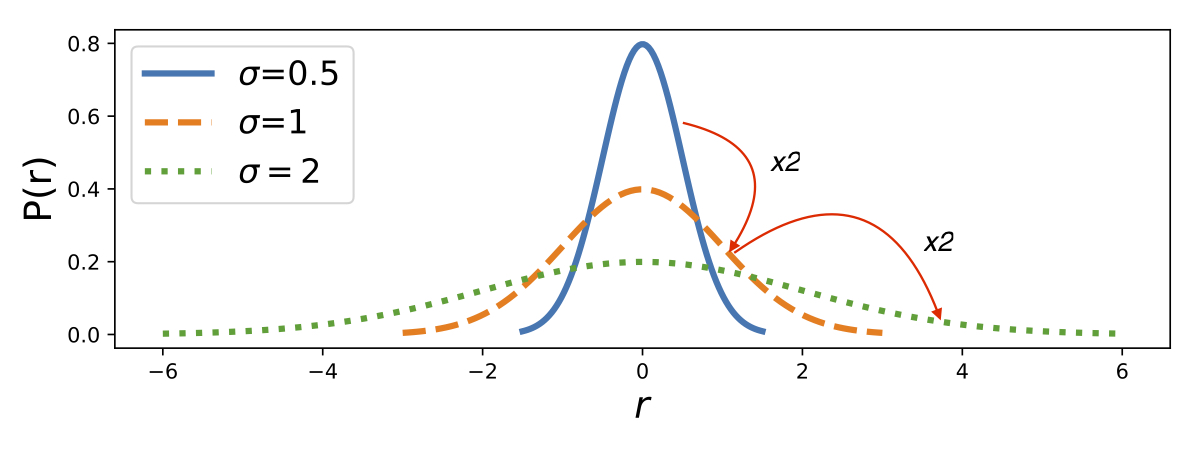
\includegraphics[width=0.8\linewidth]{ill/std_2.jpg}
  \vspace{-5pt}
  \caption{Illustration of the obfuscation effect brought by larger values of standard deviation $\sigma$.}
  \vspace{-5pt}
  \label{fig:std}
\end{figure} 

For the high utility of the obfuscated graph, smaller values of the parameter $r_{e}$ should be favored.  
The most widely known member of generating distribution $R({\sigma})$ is the truncated normal distribution with mean 0 and variance $\sigma^2$. 
In principle, $R$ could be any distribution.
As the standard deviation $\sigma$ decreases, a greater mass of $R_{\sigma}$ will concentrate near $r_{e}=0$.  
As illustrated in Figure~\ref{fig:std}, smaller values of $\sigma$ generally contributes towards better utility preserving, while at the same time they provide lower level of obfuscation. 
Larger values of $\sigma$ have the opposite effect.
Then, the amount of injected noise and consequent structural distortion will be smaller. 
Aiming at the high utility, {\soaName} aims at injecting the minimal amount of uncertainty need to achieve the necessary obfuscation. 
As outlined in Algo~\ref{alg:obf}, it computes the minimal amount of uncertainty via a binary search on the $\sigma$ value. 
\begin{algorithm}
    \begin{algorithmic}[1]
    	\item[] {\textbf{Input:}~Graph $\mathcal{G}$, obfuscation level $k$, tolerance parameter $\epsilon$}
        \item[] {\textbf{Output:}~The result $\mathcal{G}_{obf}$}
     	\STATE {$\sigma_{l} \leftarrow 0$; $\sigma_{u} \leftarrow 1$} \\
        \REPEAT
        \STATE{$\langle \hat{\epsilon}, \hat{\mathcal{G}} \rangle$ $\leftarrow$ \textbf{genObf}(-,$\sigma_{u}$)} \\
        \STATE{{\bf if} $\hat{\epsilon}=1$ (fail) {\bf then} $\sigma_{l} \leftarrow \sigma_{u}$; $\sigma_{u} \leftarrow 2\sigma_{u}$}
        \UNTIL{$\hat{\epsilon} \neq 1 $} \\
        \REPEAT
        	\STATE {$\sigma_{mid} \leftarrow (\sigma_{u}+\sigma_{l})/2$}
            \STATE{$\langle \hat{\epsilon}, \hat{\mathcal{G}} \rangle$ $\leftarrow$ \textbf{genObf}(-,$\sigma_{mid}$)}
            \STATE {{\bf if} $\hat{\epsilon} =1$~{\bf then}~$\sigma_{l} \leftarrow \sigma_{mid}$}\\
            \STATE {{\bf else} $\sigma_{u} \leftarrow \sigma_{mid}$;~~{$\mathcal{G}}_{obf} \leftarrow \hat{\mathcal{G}}$}
        \UNTIL{$\sigma_{u}-\sigma_{l}$ is enough small}
        % \COMMENT{\textcolor{blue}{\scriptsize Binary search for better obfuscation}}
        \STATE {return $\mathcal{G}_{obf}$}
    	\caption{The obfuscation algorithm}
	 \label{alg:obf}
    \end{algorithmic}
\end{algorithm}


The function {\genobf} determines the search flow. The function {\genobf} handles the search of {\keobf} instances using a given standard deviation parameter $\sigma$. It either returns the found sanitized instance or failure sign.
The search starts with an initial guess of an upper bound $\sigma_{u}$, which is iteratively doubled until a {\keobf} instance is found. Then, the binary search is performed over the range $[0,\sigma_{u}]$. The binary search terminates until the search interval is sufficiently short. The algorithm outputs the best found sanitized output  (the last one that was successfully generated; the one with the samllest $\sigma$).

\subsection{Genobf Function}
It is a difficult problem to find {\keobf} sanitized solutions using a given parameter $\sigma$ over the intractable search space. 
The function {\genobf} separate the search process into running two independent modules: (1) uncertain noise generative models and (2) privacy tests. 
The first constructs a utility-preserving noise generative model. 
By contrast, the privacy test aims to safeguard the privacy of generated obfuscation. 
It utilizes the random search to alleviate the combinational intractability.  
Multiple randomized attempts are performed. 
Every obfuscated output is subject to this privacy test. 
Iff all the attempts fail, {\genobf} returns failure sign. Otherwise, it returns the found {\keobf} instance.  

Each construction attempt begins with selecting a subset of edges subject to alteration. 
Then, it assigns the deviation among selected edges and injects uncertainty. 
While, the randomization process heavily relies on the heuristic.  
In particular, {\soaName} suggests calibrating the perturbation applied to an edge $e$ according to the ``uniqueness" of the two nodes $u$ and $v$. 
In brief, if both $u$ and $v$ are common nodes {\wrt} the property, then $r_{e}$ should be very small; 
on the other hand, if $u$ and $v$ are outliers, then $r_{e}$ should be higher. 
Meanwhile, edges need to be sampled with the higher probability if they are adjacent to outliers. 

\subsection{Limitations} 
The {\soaName} method achieves the desired level of obfuscation with the small change in the graph data, thus maintaining high utility.
However, this method has two critical weaknesses in the probabilistic context:
(1) The design heavily tailored towards the deterministic scenario {\eg} it assumes the existence of edges is binary (0,1). Thus, it fails to handle uncertain graphs where the existence of edges is probabilistic. 
All the operators, including edge selection and alteration, need to be integrated with possible world semantics carefully.
(2)  Its scheme does not consider the structural relevance of edges in critical edge selection/alteration steps, which leads to unnecessary structural distortion.
We are left asking the following questions, \emph{how to generalize existing methods to the probabilistic context?} and \emph{how to get a better trade-off between privacy and utility in the probabilistic context?} 
\section{Privacy Via {\methodName}}
\label{sec:method}
In this section we describe our algorithm, {\methodName}, which injects uncertainty to the given uncertain graph so that it becomes {\keobf} while preserving as much the stochastic nature as possible. 
A key feature of our method is to seamlessly integrate edge uncertainty and possible world semantics into the core of anonymization operators.
% 

\subsection{Heuristic for Edge Perturbation}
Edge selection is often considered as the most central operation in graph anonymization, as well as the most complex one. 
It needs to balances privacy gain and structural distortion. 
For the graph, it often needs to consider of the exponential number of edge combinations. 
Recently, the most popular paradigm for solving such problems has been using a class of heuristics. 

Successes of this approach include
(1) anonymity-aware ones that suggest injecting more considerable noise to unique nodes~\cite{Ying2009,Boldi_Injecting_2012,Hay_Anonymizing_2007} 
(2) utility-aware ones that avoid distortion over “bridge” edges whose deletion/addition would significantly impact the graph structure~\cite{Wang2011,Ninggal_Utility_2015}. 
The judicious edge selection must involve two types of heuristics which complement each other. 
Individually, they are far less effective. 
However, they have not been explored yet in the context of uncertain graphs.

Motived by the above, we first generalize the calibration of uniqueness with the marriage of KL-divergence function. 
Second, we propose a generalized version of edge relevance from an information-theoretic perspective.
Besides, we develop an efficient algorithm for its evaluation.
And, we show the use of multi-heuristics boosts anonymization efficiently and straightforwardly.

\textbf{Generalized Uniqueness}~~
The uniqueness criterion was used to measure how unique a given node is among all the nodes in the graph {\wrt} a specific property $P$. 
For a given node $v$, its uniqueness score is the inverse of the commonness score of its property value $w=P(v)$.
And, the commonness score of $w$ amounts to the weighted average distance among all other property values.

However, the conventional method merely formulates node properties as discrete values and relies on the geometric distance function to measure their distance.  
Thus, it fails to handle uncertain graphs where the property values are probabilistic.

\begin{figure}[tb]
  \centering
        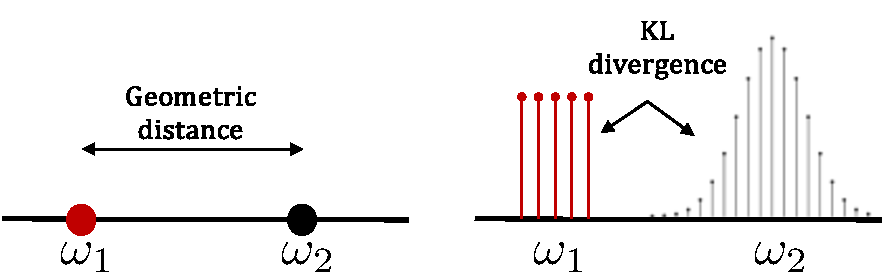
\includegraphics[width=\linewidth]{ill/shift_distance.pdf}
  \caption{The generalization of uniqueness.}
\end{figure}

We extend the preliminary version to handle the probabilistic case. 
We first systematically model uncertain property values in both continuous and discrete domains as continuous and discrete random variables, respectively.
Then, we consider the use of probability distributions, which are essential characteristics of uncertain property values, in the measuring similarity between uncertain property values. 
In this work, we use the well known Kullback-Leibler divergence to measure the distance between random variables with parameterized distributions. 

\begin{definition}
    \textbf{Uniqueness Score}
    Let $P$ be a property on the set of nodes $V$ of the input graph ,  
    let $d$ be the KL divergence function, 
    and let $\theta >0$  be a parameter. 
    Then the $\theta$-commonness of the property values $\omega$
    is $C_{\theta}(\omega)$ amounts to a weighted average over all other property values $\omega'$.    
     while the corresponding uniqueness is $U_{\theta}:= \frac{1}{C_{\theta}(\omega)}$. 
    \vspace{-5pt}
\end{definition} 
In the above definition, the weights decays exponentially as a function of the KL divergence among property values, 
and the parameter $\theta$ determines the decay rate. 
\begin{equation*}
  C_{\theta}(\omega) = \sum_{u \in V} \Phi_{\theta}(KL(\omega, P(v)))
\end{equation*}
In this work, we set $\theta=\sigma$ as the injected noise blurs the meta-distribution of property values. 
It should be noted that the commonness and uniqueness are meaningful only as relative measures. 
 
\textbf{Generalized Edge Relevance}~~
Alteration over a single edge would produce local structural change and send ripples through the rest of the graph. 
Even with the same amount of deviation, the incurred structural distortion varies on the topological role of the altered edge. 
Targets at the high utility, we should penalize edge modifications according to the incurred structural distortion.  
It naturally raises the need of measuring the relevance of edges in the probabilistic context. 

There are many potential ways to measure it. 
Importantly, the metric should be able to capture key properties of uncertain graphs.
Inspired by the importance of reliability, we measure the edge relevance of a given edge $e$ as the amount of structural distortion, measured by reliability discrepancy, caused by the unit noise subjects to the edge $e$, as follow. 
\begin{equation*}
  \begin{split}
    \mathcal{ERR}({e}) &= \frac{\Delta(\mathcal{G}+r_{e})}{|r_{e}|}  \\
                       &= \frac{\sum_{u,v} |R_{u,v}(\mathcal{G}+r_{e}) -R_{u,v}(\mathcal{G})|} {|r_{e}|}
  \end{split}
\end{equation*}

In the conventional case (deterministic graphs with edge addition and deletion $|r_{e}|=1$), it amounts to the connectivity distortion, measured by the deviation of \# of connected node pairs.  
In probabilistic graphs, $\mathcal{ERR}$ is used to generalize this concept by quantifying the stochastic impact of partial edge addition/deletion ($r_{e}$ lies in the contentious range) over the connectivity of all the possible worlds.
% It allows the estimation of structural distortion when $r_{e}$ lies in the contentious range. 
\begin{observation}
  Let $\mathcal{G}_{e}$, $\mathcal{G}_{\bar{e}}$ 
  denote two uncertain graphs that are identical to $\mathcal{G}$ with $p(e)=1$ and $p(e)=0$ respectively. 
  The reliability relevance of an edge $e$ is a constant and equivalent to 
  the following function. 
  \begin{equation}
    \mathcal{ERR}(e) = \sum_{u,v} R_{u,v}(\mathcal{G}_{e}) \big- \sum_{u,v} R_{u,v}(\mathcal{G}_{\bar{e}})
    \label{eq:err}
  \end{equation}
  Observe that, the edge relevance only depends on it topological location. 
  It amounts to the difference of the number of connected pairs between two neighbor uncertain graphs. 
\end{observation}

\textbf{Proof Sketch.}~~
According to the possible world semantics and factorization rule, we can see that   
\begin{equation*}
  R_{u,v} (\mathcal{G}) = p(e) \cdot R_{u,v}(\mathcal{G}_{e}) ~+~ \big[ 1-p(e) \big] \cdot R_{u,v} (\mathcal{G}_{\bar{e}})
\end{equation*}
Note that, the two-terminal reliability $R_{u,v}$ in $\mathcal{G}_{e}$ and $\mathcal{G}_{\bar{e}}$ are constants. 
Therefore, two-terminal reliability discrepancy introduced by the single deviation $r_{e}$ over the uncertain graph $\mathcal{G}$ is equivalent to 
\begin{equation*}
  \begin{split}
    \Delta_{u,v} (\mathcal{G}+r_{e}) ~&= r_{e} \cdot R_{u,v}(\mathcal{G}_{e}) - r_{e} \cdot R_{u,v} (\mathcal{G}_{\bar{e}})\\
    &= r_{e} \cdot ~\big[  R_{u,v}(\mathcal{G}_{e}) - R_{u,v} (\mathcal{G}_{\bar{e}})  \big]
  \end{split}
\end{equation*}
After aggregation and eliminating the factor $r_{e}$, we can see that the reliability relevance of an edge $e$ is equivalent to Equation~\ref{eq:err}. $\square$

Equation~\ref{eq:err} reminds us the basic concept of cut-edge. 
% What is the relationship between Equation~\ref{eq:err} and the conventional cut-edge definition? 
In a deterministic graph, a cut-edge is an edge of a graph whose deletion increase its number of connected components. 
We can see that the cut-edge is a binary version of $\mathcal{E}RR$.  
While $\mathcal{E}RR$ is a continuous function regarding the edge deviation $r_{e}$ and reliability discrepancy. 
$\mathcal{E}RR$ is not only relevant to connectivity discrepancy but also consider its scale.  

\textbf{Re-visiting the Computation Challenge}~~
\begin{figure}
    \subfigure[Iterative Evaluation]{\label{fig:itERR}
      \begin{minipage}[l]{0.46\columnwidth}
        \centering
        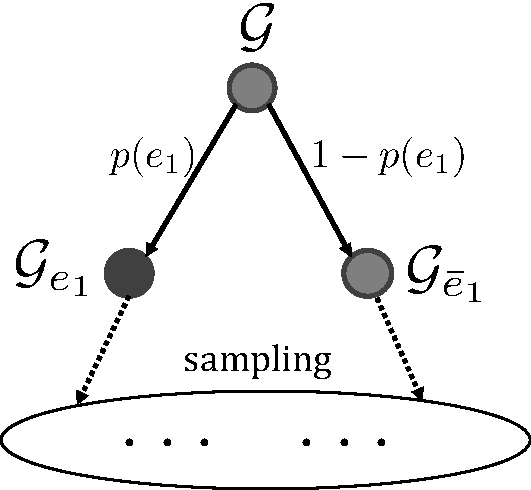
\includegraphics[height=2.6cm]{ill/iterativeERR.pdf}
      \end{minipage}
      }
    \subfigure[Memorized Evaluation]{\label{fig:groupERR}
      \begin{minipage}[l]{0.46\columnwidth}
        \centering
        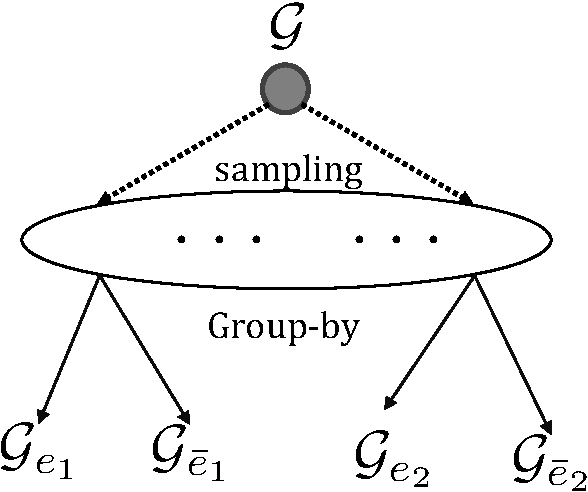
\includegraphics[height=2.6cm]{ill/groupERR.pdf}
      \end{minipage}
      }
    \caption{Sampling-based reliability detection}
    \label{fig:computationERR}
\end{figure} 
As shown in Equation~\ref{eq:err},  
the evaluation of $\mathcal{E}RR(e)$ involves a fundamental problem concerning uncertain graphs, which we call 
the Two-Terminal Reliability detection (TTR) problem. 
Since this problem is \#P-complete, we focus on efficiently and accurately approximate TTR.
The Monte-Carlo sampling method can be used to estimate the underlying reliability of an uncertain graph. 
Namely, we create a subset of possible worlds of the given uncertain graph with the use of edge sampling probabilities. 
Then, we take the average of the number of connected node pairs in the sampled worlds as an approximation. 
 
% The $\mathcal{E}RR$ evaluation over all the edges is not trivial. 
It is not trivial to evaluate $\mathcal{E}RR$ over all the edges. 
One option is to iteratively invoke the sampling-based reliability computation over all the edges, 
as illustrated in Figure~\ref{fig:itERR}. 
It is straightforward to compute the connected components of a graph in linear time (regarding the numbers of the nodes and edges of the graph) using either breadth-first search or depth-first search.
For each edge, we need to perform the connected component detection for $N$ sampled graphs.
Thus, the overall time complexity is typically in the order of $\mathcal{O}( N |E|^{2})$.
Apparently, the iterative evaluation is inefficient when the uncertain input graph is massive.

Here, we present an efficient method with the time complexity in the order of $\mathcal{O}(N |E|)$.
As illustrated in Figure~\ref{fig:groupERR}, it memories the connected components detection result of samples. 
For evaluating the reliability relevance of one edge $e$, we group the sampled possible worlds according to the edge existence, 
then get the average value of $cc$ over each group as accurate approximation of $cc(\mathcal{G}_{e})$ and $cc(\mathcal{G}_{\bar{e}})$. 
Instead of sampling and evaluation from the scratch, we utilized the memorized results. 
The running time analysis roughly follows the analysis of the single-edge case.  
By this way, we bring the evaluation of edge reliability relevance to the realm.

\textbf{Edge Selection Boosted by Multi-heuristics}~~
To get the balance between anonymity and utility, we combined the generalized uniqueness metric $U$ and relevance $R$ metric by taking the ratio between them. 
We denote the combination as Balance Factor (BF) which is defined as follows:
\begin{equation*}
    BF(v)=\frac{U(v)}{R(v)}
\end{equation*}
For a give vertex $v$, $U(v)$ is the normalized uniqueness score of its property value among all the node in the original graph; $R(v)$ is the sum of reliability relevance of edges adjacent to the vertex. 
The higher value of BF represents the better trade-off between anonymity preserving and utility preserving. 
Our algorithm uses this heuristic to select and perturb the edge of uncertain graphs, as outlined in Algorithm 2. 




 % hybrid Heuristic
\subsection{Stochastic Uncertainty Injecting Scheme}
For each sampled edge $e$ with the distributed standard deviation $\sigma_{e}$, we select the probability deviation $r_{e}$ where $r_{e} \leftarrow R_{\sigma_{e}}$. 
Thus, the remaining question is \emph{how can we safely alter edge probability for higher anonymity?}
Given the deterministic graph, the idea of uncertainty injecting is to transfer probabilities from existing edges to potential edges, as outlined in Equation~1.
However, the uncertainty injecting scheme is unexplored in the uncertain scenario.  
\begin{figure}[!htb]
  \centering
        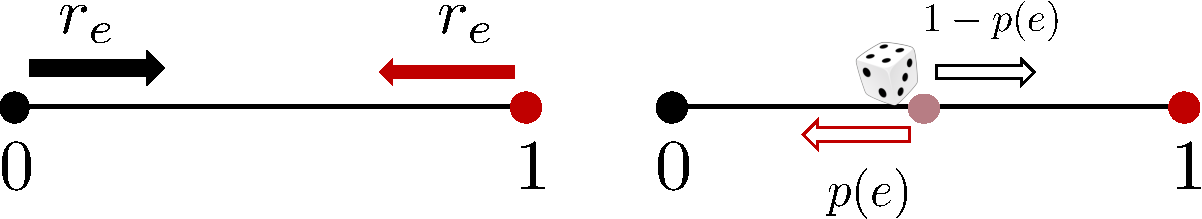
\includegraphics[width=\linewidth]{ill/shift_UI.pdf}
    \caption{The generalized uncertainty injecting scheme.}
\end{figure}
There are many potential ways to extend the uncertain injecting scheme to the probabilistic context.   
One option is the Most-Provable-Scheme where the edge probability alteration follows the most probable policy.
\begin{equation*}
  p(e) =
  \begin{cases}
     p(e)-r_{e}    & p(e) \ge 0.5 \\
     p(e)+r_{e}    & otherwise 
  \end{cases}
  \label{eq:inject}
\end{equation*}

Another simple alternative is to consider the probability the edge exists as an indicator of the scheme. 
It performs the following uncertainty injecting scheme.
\begin{align}
  p(e)~&=~ [p(e)] \cdot (1-r_{e})+ [1-p(e)] \cdot r_{e} \\
      ~&=~ p(e) + \big[ 1- 2 p(e) \big] \cdot r_{e}
  \label{eq:ui}
\end{align}
It has already been used as the uncertainty injecting scheme in our previous work~\cite{Xiao:2018}; 
The flexible value of the edge probability is limited to the range between $p(e)$ and $1-p(e)$.
Intuitively, it requires maximizing degree entropy/variance. 
% The intuitive interpretation is XXXXX. 

However, its connection to the core anonymity objective and the mathematical foundation are unclear. 
In this work, we show the stochastic uncertainty injecting scheme can maximize the related objective function of anonymity.  

\textbf{The relaxed version of anonymity}~~
To simplify the discussion, let us consider the primary case $k$-obf which low bounds the entropy of posterior-probability distribution over all the nodes.  
It imposes a set of hard constraints on the output solution. 
To make it formal, let us define the set of feasible solutions satisfying all the constraints as:
\begin{equation*}
  \{\pg~~s.t.~~ \forall v ~\mathrm{E}(v) \ge  \log k \}. 
\end{equation*}
$k-$obf can be expressed as joint satisfaction of a set of constraints 
since the uncertain graph is said to be $k$-obf iff it $k-$obfuscates all the nodes. 
Then, in order to sanitize graph, we could maximize the following function: 
\begin{equation*}
    \mathcal{F}_{e} = \prod_{v \in V} \mathcal{C}_{v}              
\end{equation*} 
where 
\begin{equation*}
  \mathcal{C}_{v} = 
  \begin{cases}
    1 & \mathrm{E}_{v} \ge  \log k \\ 
    0 & otherwise 
  \end{cases}
\end{equation*}

The single constraint {\Constraint} is either fully satisfied or thoroughly violated. 
The discontinuity limits the opportunity of gradient-based optimization methods.
The connection between our objective function is still unclear.  
Thus, we relax the single constraint {\Constraint} to a fuzzy relation as: 
\begin{equation*}
  \mathcal{C}_{v} = e^{\mathcal{E}_{v}-\lambda}.
\end{equation*}
Then, the satisfaction becomes a continuous and differential function {\wrt} the entropy. 
It turns out that the problem can be reduced to maximizing a much simpler function with the relaxed version of anonymity.  

\begin{observation}
  The maximization of $\mathcal{F}_{e}$ is equivalent to the maximization of the following function:
  \begin{equation*}
    \mathcal{F} =  \sum_{v\in V} E(v) - \Number E(\Omega)
  \end{equation*}
\end{observation}
Targeting at high utility, it aims at increasing the uncertainty at the vertex level $\sum_{v \in V} E(v)$. 

\textbf{Proof Sketch.}~~
Let $\Omega$ presents the domain of property values in the given graph; we can see that 
\begin{equation*}
  \mathcal{F}_{e} = \prod_{\omega \in \Omega} \underbrace{\mathcal{C}_{\omega} \ldots \mathcal{C}_{\omega}}_{s(\omega)}, 
\end{equation*}
Taking logarithm for both sides and combining the approximation, our goal is actually to maximized 
\begin{align*}
  \log \mathcal{F}_{e} &= \sum_{\omega \in \Omega} s(\omega)~\log C(\omega) \\
                       &= \sum_{\omega \in \Omega} s(\omega) \big[ E(\omega) - \lambda \big] \\
                       &= \sum_{\omega \in \Omega} s(\omega) E(\omega) ~-~ \Number \lambda 
\end{align*}
Therefore, after removing the constant $\Number\lambda$, our goal is actually to maximize 
$\sum_{\omega \in \Omega} s(\omega) E(\omega)$. 
It bridges the anonymity of the overall graph $\mathcal{F}_{e}$ 
with the component coding (the disorder) of the fuzzy matching matrix. 

To perform data coding, we have two angles, row  and column, that gain the same result of coding length $\mathcal{L}$ as:
\begin{align*}
  \mathcal{L} &= \sum_{v \in V} E(v) + \Number \log \Number                             &(row)\\
              &= \sum_{\omega \in \Omega} s(\omega) E(\omega)~+~\Number E(\Omega) &(column). 
\end{align*}
Therefore, after removing the constant $\Number \log \Number$, our goal is actually to maximize 
$\mathcal{F}_{e}$. $\square$  

\begin{observation}
  Equation~\ref{eq:ui} approximates the gradient-based exploration of the simplified objective function $F$.
\end{observation}

\textbf{Proof Sketch.}~~
Fix such node $v \in \mathcal{G}$ and let $e_{1},\ldots, e_{l}$ be $l$ edges that include $v$. 
Letting $d_{v}$ be the random variable corresponding to the degree of $v$, 
we have 
\begin{equation*}
  d_{v} ~=~ \sum_{i}^{l} p(e_{i}). 
\end{equation*}
As ever described, {\methodName} selectively modifies edges connected to unique nodes ({\ie}, nodes with high degree).
The degree of such node $v$ can be approximated by the normal distribution. (The Central Limit Theorem becomes effective already for $l\approx 30$; for unique nodes in the real uncertain graph, the approximation becomes accurate enough.) We have
\vspace{-5pt}
\begin{align*}
   d_{v}~&\sim~\mathcal{N}(u, \sigma^2); \\
   \sigma^{2}~&=~\sum_{i=1}^{l} Var(P(e_{i}))=\sum_{i=1}^{l} p(e_{i}) (1-p(e_{i}))
   \vspace{-15pt}
\end{align*}
The entropy of the random variable, $E(v)$, can then be approximated by the differential entropy of the normal distribution as ${{1}\over{2}}{\ln (2\pi\sigma^2)}+ {{1}\over{2}}$. 
The gradient of our objective function {\wrt} the edge existence  can be rewritten as
\begin{align*} 
  \nabla \mathcal{F}~&=~\nabla E_{v}~=~\nabla \ln(\sigma^2) \\
                    ~&\sim \frac{1}{\sigma^2} \nabla \sigma^{2}~\sim~\frac{1}{\sigma^2} \big [ 1-2~p(e_{i}) \big].~\square
\end{align*} % uncertainty Injecting 
\subsection{The {\methodName}-obf Algorithm}
\begin{algorithm}[!htb]
	\begin{algorithmic}[1]
    	\item[] {\textbf{Input:}~Uncertain graph $\mathcal{G}$, the desirable obfuscation level $k$, \
                tolerance parameter $\epsilon$, the standard deviation $\sigma$, $t=5$ five attempts and auto tuned size multiplier $c$.}
        \item[] {\textbf{Output:}~A pair of the sanitized output $\mathcal{G}_\text{obf}$ and $\hat{\epsilon}$.}
        \STATE {Compute the generalized uniqueness score $U$}
        \STATE {Compute the reliability relevance $R$}
        \STATE {Get $\mathcal{H}$:~$\frac{\epsilon}{2}\Number$ nodes with highest $U(v)R(v)$ score}
        \STATE {Compute and normalize balance factor $BF(v)=\frac{U(v)}{R(v)}$}
        \STATE {$\hat{\epsilon} \leftarrow 1$}
   		\FOR{$t$ times} 
         	\REPEAT  
                \STATE {$E_{C} \leftarrow E$} 
            	\STATE{randomly pick a vertex $u \in V \setminus \mathcal{H}$ according to $BF$}
            	\STATE{randomly pick a vertex $v \in V \setminus \mathcal{H}$ according to $BF$}
                \IF {$(u,v) \in E$}
                    \STATE {$E_{C} \leftarrow E_{c} \setminus \lbrace(u,v)\rbrace$ with the probability $p(e)$}
                \ELSE
                    \STATE {$E_{c} \leftarrow E_{c} \cup \lbrace(u,v)\rbrace$}
                \ENDIF
            \UNTIL{$E_{C}=c|E|$}
            \FORALL {$e \in E_{C}$} 
            	\STATE {Compute $\sigma(e)$}
                \STATE {Generate $r_{e} \leftarrow R_{\sigma(e)}$}
                \STATE {Inject uncertainty: $p(e) \leftarrow p(e) + \big[ 1- 2 p(e) \big] \cdot r_{e}$}
            \ENDFOR
            \STATE {$\epsilon_{s} \leftarrow anonymityEvaluation(\mathcal{G}_{s})$ }
            \IF {$\epsilon_{s} < \text{min}(\hat{\epsilon},\epsilon)$}
                \STATE {$\hat{\epsilon} \leftarrow \epsilon_{s}$, $\mathcal{G}_\text{obf} \leftarrow \mathcal{G}_{s}$}
            \ENDIF 
        \ENDFOR 
        \STATE {return $\langle \hat{\epsilon},  \mathcal{G}_\text{obf} \rangle$}
      	\caption{Squid-genObf}
        \label{alg:squid}
    \end{algorithmic}
\end{algorithm}

The {\methodName}-obf performs following steps to judiciously use the ``uncertainty budget" $\sigma$.

[Line 1-2]~It computes the uniqueness and relevance level for each vertex $v \in V$. 
The more unique a vertex is, the harder it is to obfuscate it. 
The more relevant a vertex is, the more significant impact the mutation brings.

[Line 3]~It first select the set $\mathcal{H}$ of $\frac{\epsilon}{2}\Number$ nodes, and exclude them from the subsequent mutation effort. Instead of excluding the nodes requires most considerable mutations (uniqueness), {\methodName}-obf also excludes the ones with significant structural relevance. 

[Line 4]~The mutation over edges is needed to obfuscate the set of nodes not in $\mathcal{H}$. 
Higher uncertainty is necessary t obfuscate  ``outliers", nodes with higher uniqueness score. 
Thus, edges need to be sampled with the higher probability if they are adjacent to unique nodes. 
Mutation over ``bridge-like" edges need to be minor to preserve data utility. 
Thus, edges with higher relevance score need to be sampled with lower probability.
We utilize two complementary heuristics, uniqueness (the anonymity-aware one) and relevance (the utility-aware one) to guide our edge selection and mutation. 
In particular, it assigns a probability to every $v \in V$ which is proportional to the balance factor $BF(v)$ of $v$. 










\section{Empirical Study}
\label{sec:ex}
We evaluated the performance of {\methodName} in comparison with the Rep-based Anonymization (RA) and the Casting-based Anonymization (CA) methods.

Recall that the RA method first extracts a single representative deterministic instance 
via algorithms proposed by Parchas~{\etal} in~\cite{Parchas_Gullo_Papadias_Bonchi_2014}.
Then, RA utilizes the deterministic graph anonymization method~\cite{Boldi_Injecting_2012} to produce the sanitized output.
While, the CA method first casts the given uncertain graph into a weighted deterministic graph.
Then, CA utilizes the weighted graph anonymization method, proposed by Sudipto~{\etal}~\cite{Das_Anonymizing_2010} to generate the corresponding sanitized output. 
Finally, it re-casts the output to the probabilistic version.

\begin{figure*}[!htb]
    \centering
    \subfigure[PPI]{
    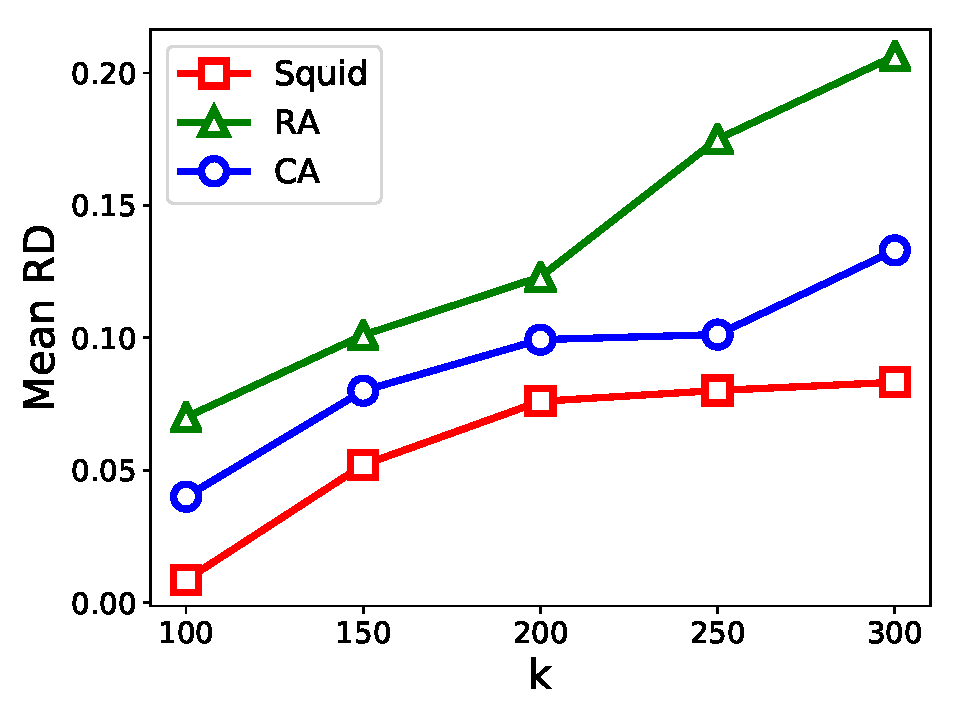
\includegraphics[width=.31\textwidth]{expResult/ppi_RD.pdf}
    }
    \subfigure[BK]{
    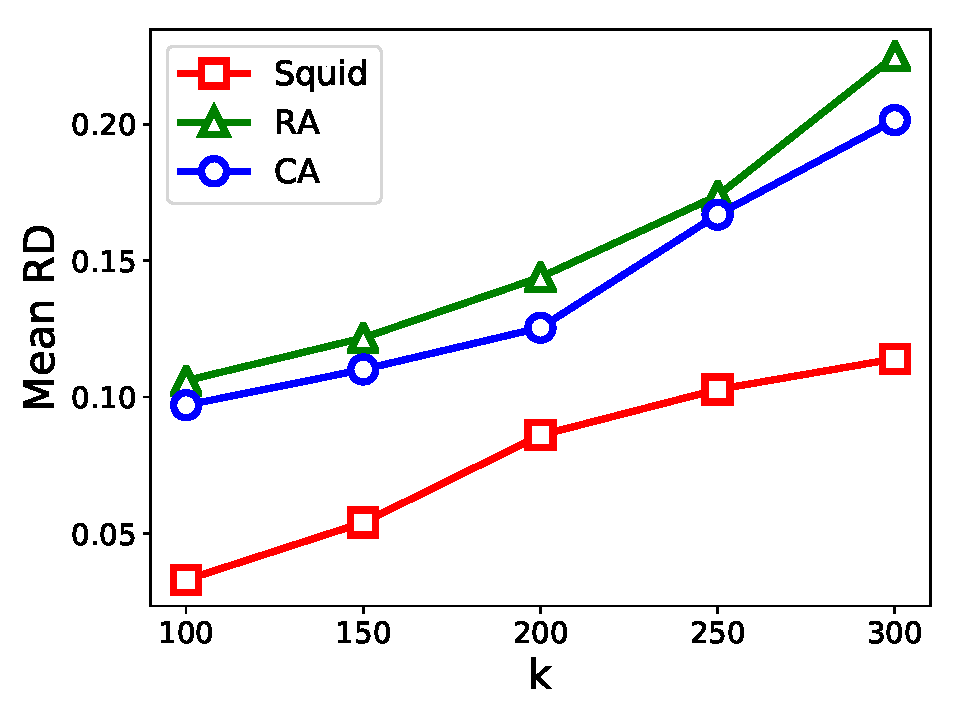
\includegraphics[width=.31\textwidth]{expResult/bk_RD.pdf}
    }
    \subfigure[DBLP]{
    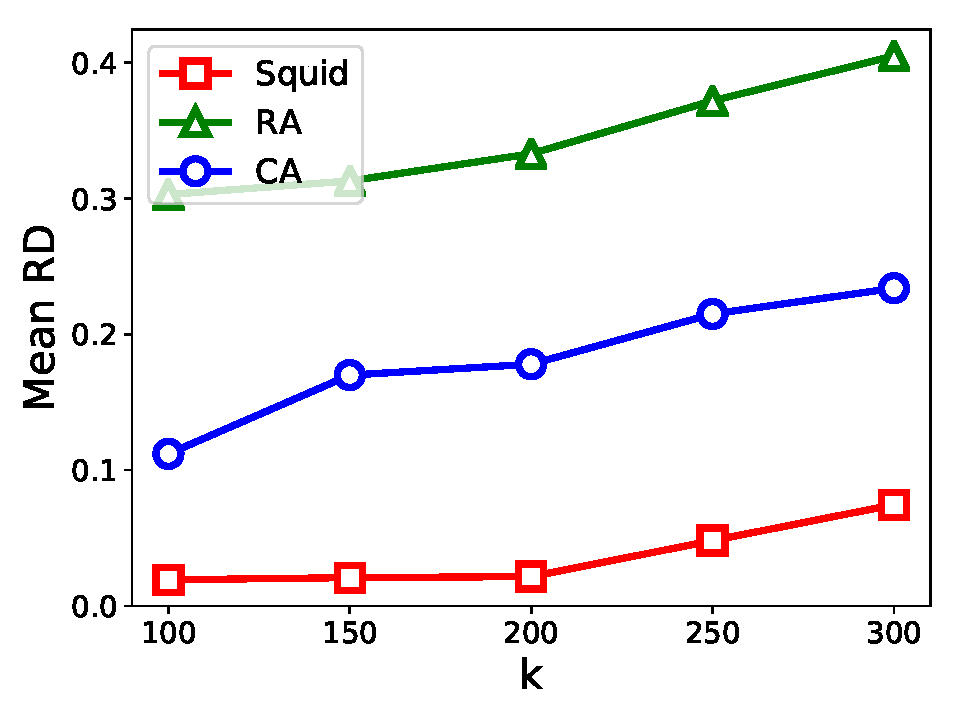
\includegraphics[width=.31\textwidth]{expResult/dblp_RD.pdf}
    }
    \vspace{-5pt}
    \caption{Reliability Discrepancy (RD) of sanitized uncertain graphs of different anonymization methods against original graphs. The smaller the discrepancy the more information of connectivity structure is preserved.}
    \label{fig:rd}
\end{figure*} 
\begin{figure*}
    \centering
    \subfigure[PPI]{
    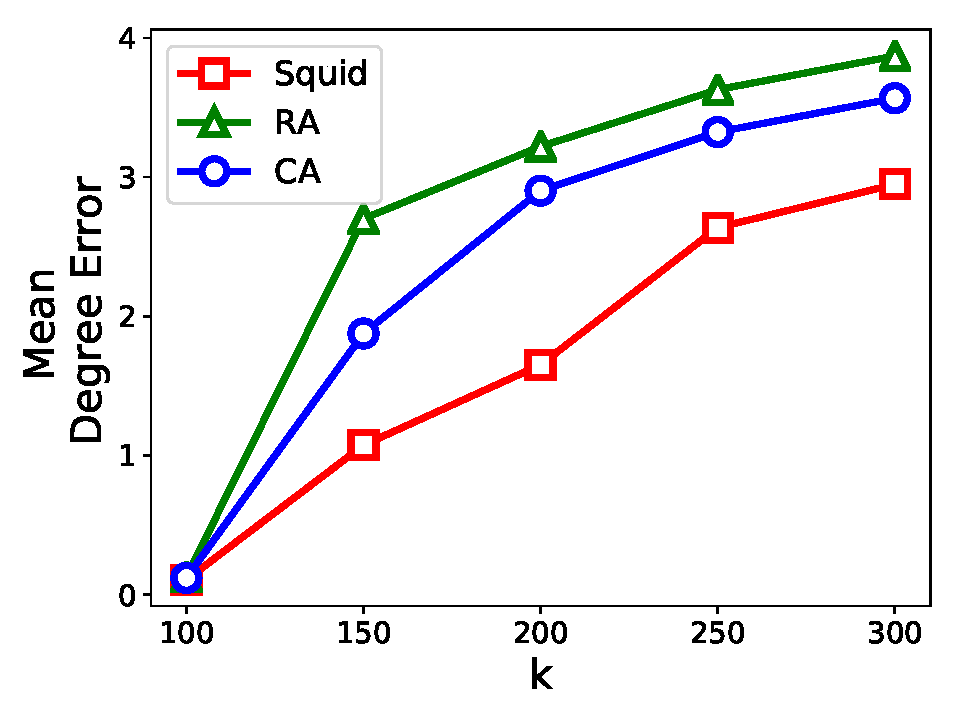
\includegraphics[width=.31\textwidth]{expResult/ppi_dd.pdf}
    }
    \subfigure[BK]{
    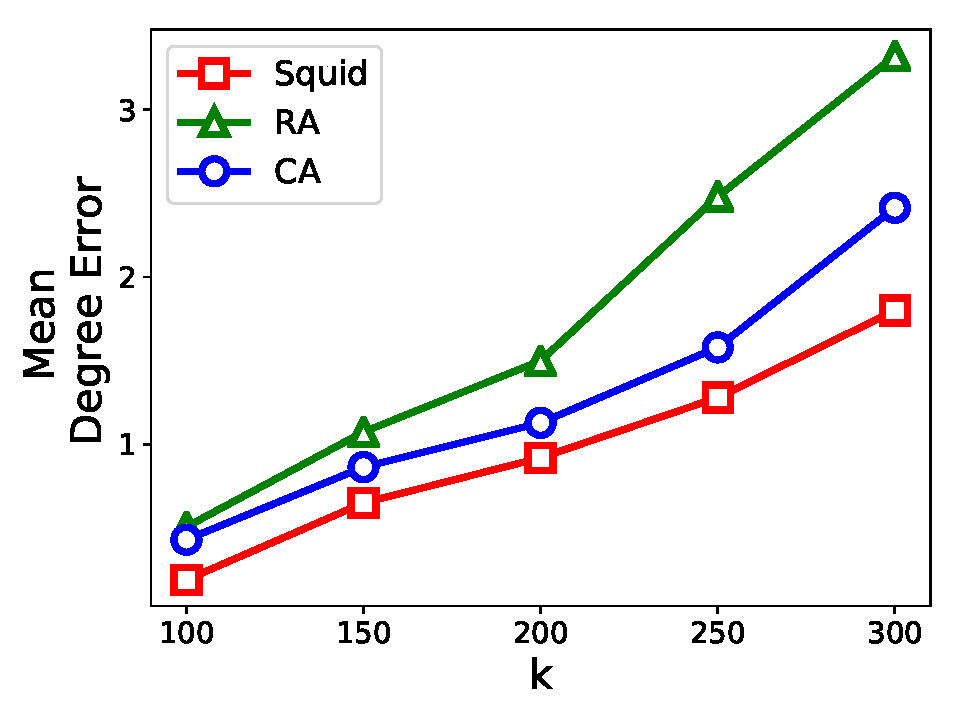
\includegraphics[width=.31\textwidth]{expResult/bk_dd.pdf}
    }
    \subfigure[DBLP]{
    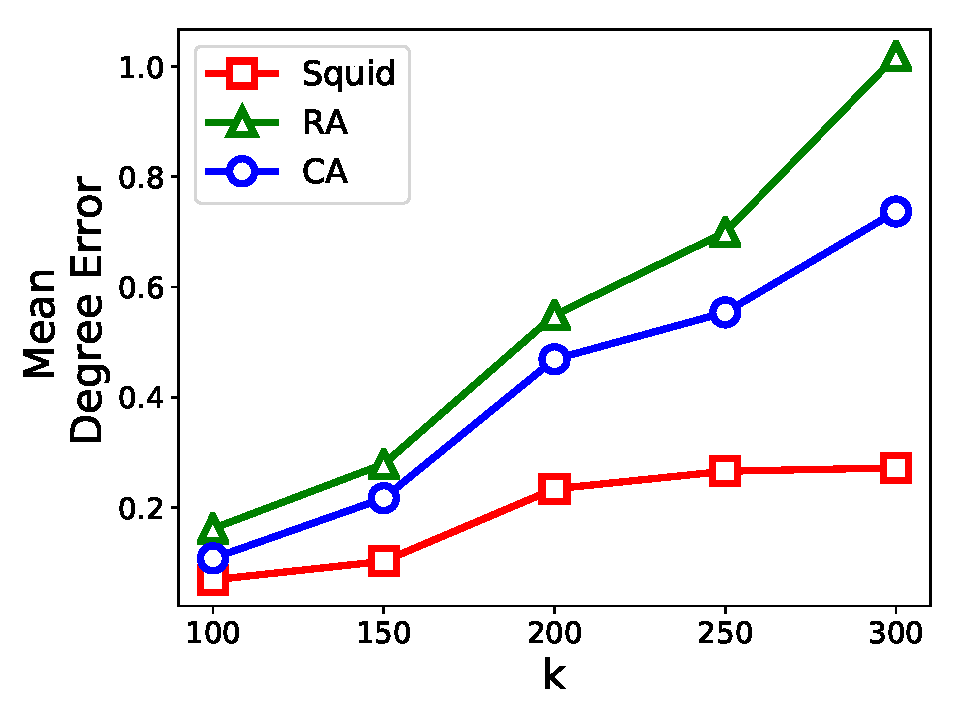
\includegraphics[width=.31\textwidth]{expResult/dblp_dd.pdf}
    }
    \vspace{-5pt}
    \caption{Degree error of sanitized uncertain graphs of different anonymization methods on three real graphs. The smaller the degree error the more information of degree distribution is preserved.}
    \vspace{-9pt}
    \label{fig:dd}
\end{figure*} 
\subsection{Experiment Settings}

% \begin{table}[t]
%     \centering
%         \caption{Characteristics of datasets and privacy parameters}
%     \scalebox{0.75}{
%         \begin{tabular}{l|c|c|c|c||c}
%         \hline 
%         \textbf{Name} & \textbf{Content}  & \textbf{Nodes}    & \textbf{Edges}    &\textbf{Edge Prob}     & \textbf{$\epsilon$}\\
%         \hline  
%         \textrm{PPI} & \footnotesize{Protein-protein Interaction}  &12K       &397K       & 0.29         &$10^{-2}$\\
%         \textrm{BK}  & \footnotesize{Location-based OSN}    &58K       &214K       &0.29          &$10^{-3}$ \\
%         \textrm{DBLP}& \footnotesize{Co-authorship Network} & 824K      &5M         & 0.46         & $10^{-4}$\\
%         \hline
%         \end{tabular}
%      }
%         \label{tab:dataset}
%     \vspace{-10pt}
% \end{table}

\begin{table}[t]
    \centering
        \caption{Characteristics of datasets and privacy parameters}
    \scalebox{0.85}{
        \begin{tabular}{|l|c|c|c||c|}
        \hline 
        \textbf{Name} & \textbf{Content}  & \textbf{Nodes}    & \textbf{Edges}  & \textbf{$\epsilon$} \\
        \hline 
        \hline  
        \textrm{PPI} & \footnotesize{Protein-protein Interaction}  &12K       &397K        &$10^{-2}$\\
        \textrm{BK}  & \footnotesize{Location-based OSN}    &58K       &214K        &$10^{-3}$ \\
        \textrm{DBLP}& \footnotesize{Co-authorship Network} & 824K      &5M         & $10^{-4}$\\
        \hline
        \end{tabular}
     }
        \label{tab:dataset}
    \vspace{-10pt}
\end{table}

\textbf{Datasets}~~We test them on three uncertain graphs: PPI, BrightKite (BK) and DBLP as described in Table \ref{tab:dataset}. They have been widely used in the study of uncertain graphs~\cite{Zhao_Detecting_2014,Potamias_K_2010,Jin_Distance_2011}. 

\begin{itemize}
	\item{PPI is a dataset of protein-protein interactions, provided by Disease Module Identification DREAM Challenge. The probability of any edge corresponds to the confidence that the interaction actually exists, which is obtained through biological experiments.}
	\item{Brightkite is a location-based social network. In this dataset, each node represent a user. The probability of any edge corresponds to the chance that two users visit each other.}
	\item{DBLP is a dataset of scientific publications and authors. Each node represent an author. Two authors are connected by an edge if they have co-authored in a project. The uncertainty on the edge denotes the likelihood that the two authors will collaborate in a new project.}
\end{itemize}
% Answer the question why use these dataset 
DBLP dataset only has a few probability values, while probability values of Brightkite  are generally very small. The PPI dataset has a more uniform probability distribution. We also present their degree distributions of “unique” nodes (with high degree and obfuscation level is smaller than 300). Observe that, all the three graphs have a heavy-tailed degree distribution. Namely, they are difficult to be obfuscated.

\textbf{Parameter Setting}~~We consider the obfuscation level $k$ in the range $[100,300]$, and possible tolerance values $\epsilon$ to explore their performance difference. 

\textbf{Statistics}~~For every obfuscated result, we sampled $N$ possible worlds to compute its statistics of interest. Note that it has been shown that 1000 possible worlds usually suffices to achieve accuracy converge.  Here, we report their discrepancy against the original one. The smaller discrepancy, the better uncertain graph data utility preserving.



\subsection{Uncertain Graph Statistic Preserving}
In the set of experiment, we focus on evaluating their performance concerning statistic preserving. 
The evaluation includes two groups of graph statistics. 
The first group includes node separation statistics that quantify the interconnectivity and density of the overall graph.   
This group includes metrics such as Shortest Path Length~\footnote{In particular, we use Hyper ANF~\cite{Boldi_Rosa_Vigna_2011} to approximate shortest path-based statistics.},Reliability and Graph Diameter. 
The second group includes degree-based statistics such as Average  Node Degree and Degree Distribution.
These topological statistics that characterize how degrees are distributed among nodes. 
Our results are highly consistent across our pool of graph statistics.
For brevity, we report only Reliability, Shortest Path Length and Node Degree as their representatives. 

\textbf{Node Separation Statistic.} 
We plot the connectivity distortion introduced by anonymity process in Figure~\ref{fig:rd}.  
As expected, larger $k$ introduced more significant connectivity distortion, because more noise was added to achieve the desired level of anonymity.   
These observations are consistent across biological and social uncertain graphs.

There is a clear improvement of {\methodName} over CA and RA methods for the integration of possible world semantics and uncertain-aware search strategy. 
For example, in all the dataset ($k=300$), the reliability discrepancy introduced by {\methodName} is well below 0.1 whereas the ones added by CA is below 0.2. The reliability discrepancy introduced by RA on PPI, BK, DBLP is around 0.2, 0.2, 0.4 respectively. We also observe that as the size of graph increases (PPI $\rightarrow$ DBLP), the performance gap becomes larger and larger.

Note that CA and RA schemes deteriorate data utility due to the disregarding the possible world semantics. 
For example, in the case, $k=100$ (weak privacy guarantee required little noise), CA and RA incur relatively large connectivity distortion. 
The representative extraction step of RA introduces noise and results in cumulative errors in the anonymization step. Consequently, sanitized results differ from the original ones. 
The CA scheme fails to reflect the connectivity of uncertain graph correctly. Therefore, it produces inferior results even with the focused anonymization strategy. 


\textbf{Degree-based Statistic.}~Figure~\ref{fig:dd} shows the error of Node Degree values on PPI, BK and DBLP compared to their sanitized outputs. 
The obfuscated output of {\methodName}, CA capture well Node Degree in all datasets; 
our method {\methodName} is consistently better.    
In the largest dataset DBLP, the degree error $0.2$ is much lower than $1.08$ imposed by the two-phase anonymization scheme (RA) in the same level of obfuscation ($k=300$).  
As with previous experiments, the performance gap increases as the graph size increases.

\textbf{Summary.} 
Our experimental results show that sanitized outputs generated by {\methodName} exhibit structural features close to those of their original uncertain graphs. 
Results show that we are able to effectively balance the utility and privacy in the probabilistic graph context.
The result is encouraging because we can eliminate the noise by moving from the reliability model to a more accurate graph model incorporating with the possible world semantics.
\begin{figure*}
    \vspace{-5pt}
    \centering
    \subfigure[PPI]{
    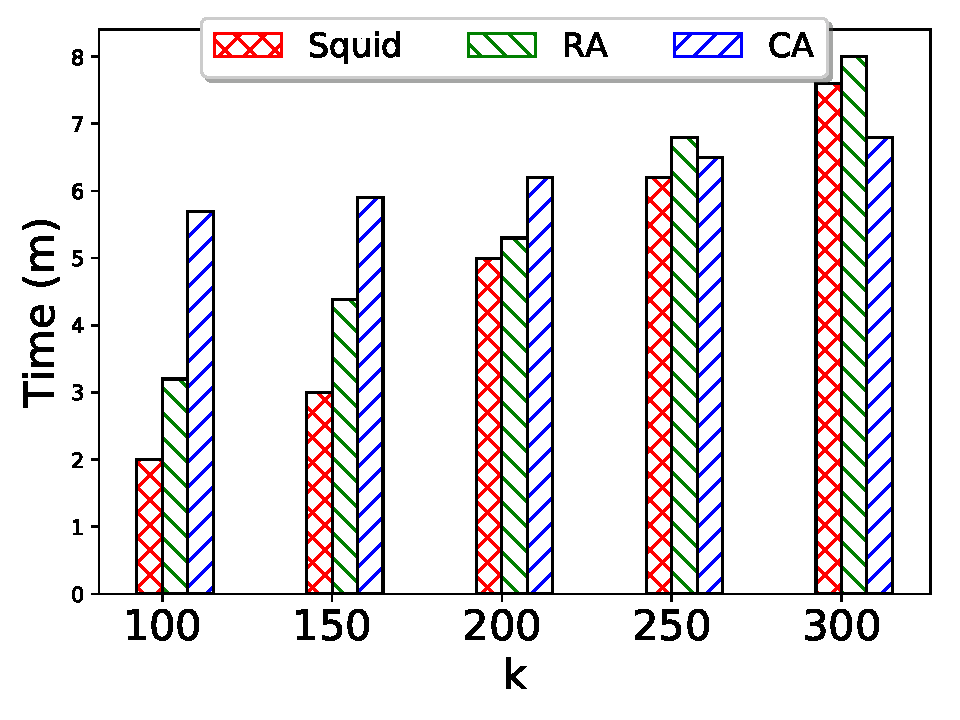
\includegraphics[width=.30\textwidth]{expResult/ppi_time.pdf}
    }
    \subfigure[BK]{
    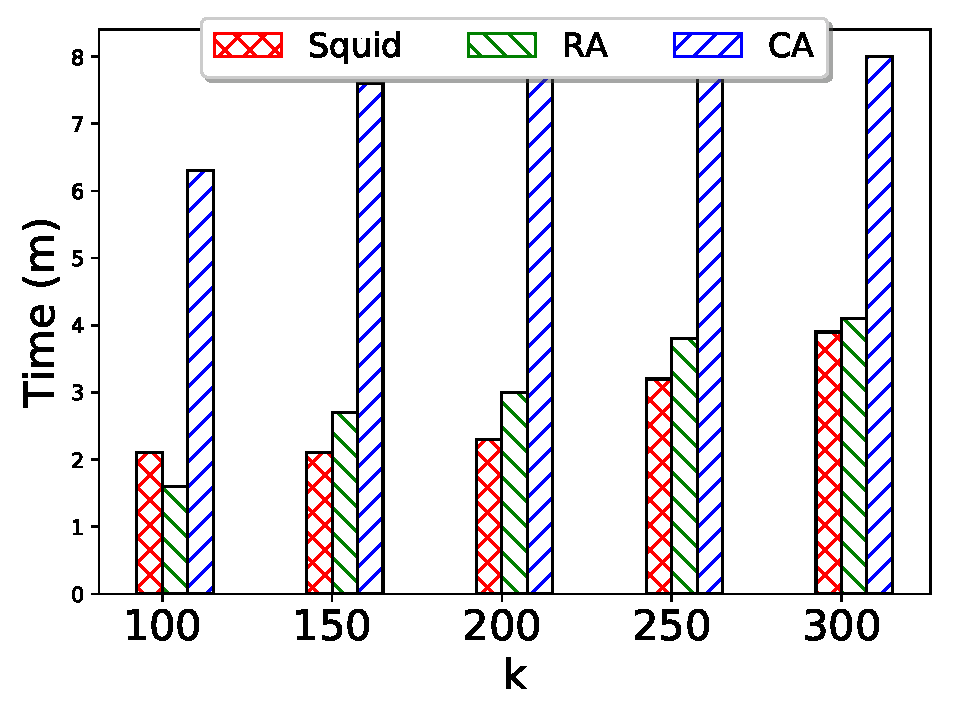
\includegraphics[width=.30\textwidth]{expResult/bk_time.pdf}
    }
    \subfigure[DBLP]{
    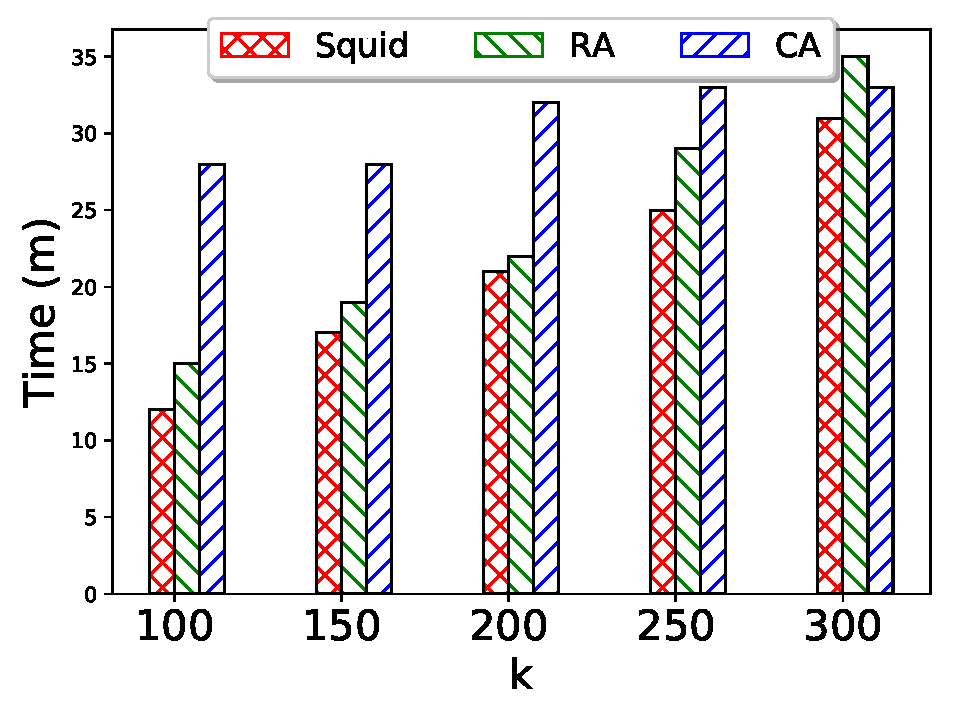
\includegraphics[width=.30\textwidth]{expResult/dblp_time.pdf}
    }
    \vspace{-5pt}
    \caption{Time efficiency of different anonymization methods on three real graphs.}
    \label{fig:time}
    \vspace{-10pt}
\end{figure*}
\subsection{Uncertain Graph Application Measures}
\begin{figure}[!htb]
    \centering
    \subfigure[PPI]{
    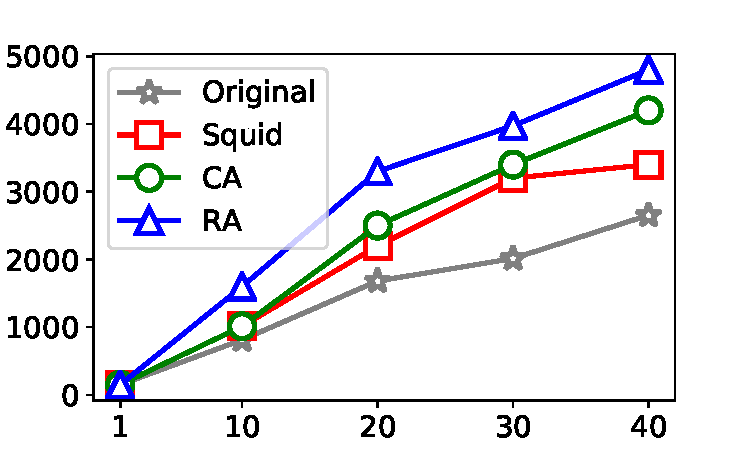
\includegraphics[height=4cm]{expResult/ppi_IM.pdf}
    }
    \subfigure[BK]{
    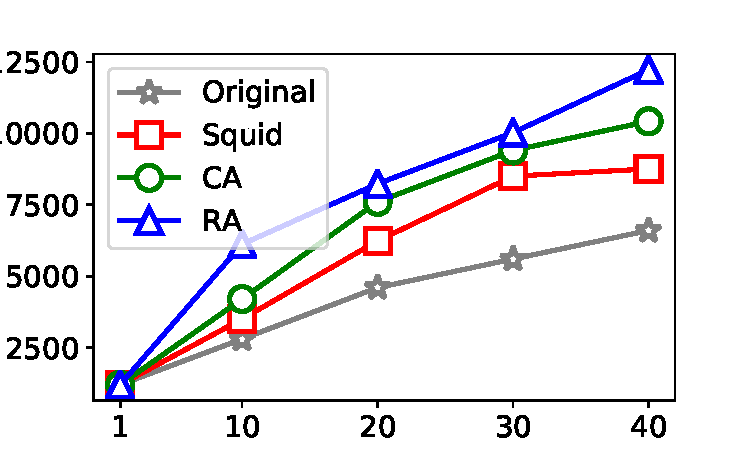
\includegraphics[height=4cm]{expResult/bk_IM.pdf}
    }
    \caption{ Results of the influence maximization algorithm on PPI and BK datasets, compared to sanitized outputs where $k$=100.}
    \vspace{-15pt}
    \label{fig:IM}
\end{figure} 
For a sanitized graph to be meaningful for research use, it should produce 
the close results as the original graph in the application-level settings. 
Influence Maximization is known as essential techniques with advertisement and public relation campaigns.
It tries to locate users in the network who can most quickly spread information through the network. 
Usually, related algorithms start with identifying the nodes which can maximize influence and model the spread of influence through network how many users has ultimately reached.  
Motivated by these facts, we compare the result of influence maximization on sanitized outputs and original graphs. 
In general, it enables us to quantify the trade-off between application utility and privacy protection. 

\textbf{Methodology.}~We used the sampling method to get the expectation value of influence. For each sampled graph, we adopt the degree discount method (a heuristic-based method with light computation) to find the most influential nodes (seeds) on a deterministic graph. Starting from those seeds, we run the weighted cascade influence dissemination model to determine the number of reached users in the network. 

For the limit of computation resource (memory overhead), we only perform the set of experiment over PPI and BK datasets. We report the expected number of reached nodes when the number of initial seeds in Figure~\ref{fig:IM}. 
There are clear and visible trends across PPI and BK datasets. 
Graphs with privacy protection diverge from the results of original graphs.
We can see that {\methodName} produces closer results with the identical privacy protection, comparison to CA and RA methods. 
Overall, our experimental assessment on influence maximization applications confirms our intuition: by incorporating the possible world semantics into the core of anonymization such as edge selection and uncertainty injecting, one can achieve the same desired level of anonymity with a smaller impact in the uncertain graph utility.  
\vspace{-6pt}
\subsection{Results on time efficiency}
These anonymization algorithms were implemented in C++ and run on Intel Core i7 CPU, 2 GHZ, 6MB cache size. We plot their running times on on tested datasets (PPI, BK, DBLP) in Figure~\ref{fig:time}. For larger values for anonymity level $k$, all the methods take more time to find the sanitized solutions. It is because the increased efforts (more noises \& more modified edges) needed to achieve the higher anonymity level (larger values of $k$). 
In comparison, our {\methodName} achieves the comparable efficiency with RA and CA methods.  

As excepted, the time efficiency of our {\methodName} is close to RA, better than CA.
{\methodName} and RA use the randomized search strategy to identify sanitized uncertain solutions using the given standard deviation $\sigma$, while {\methodName} takes a connectivity model instead of degree sequence adopted in RA. 
The computation generalized uniqueness and relevance metrics can be finished off-line.
As we mentioned, multi-heuristics can co-boost the randomized search strategy in the quite straightforward way with little extra effort. 


\vspace{-3pt}
\section{Conclusion}
In this work, we first identify the overlooked problem–uncertain graph anonymization. 
We develop a new scheme, {\methodName}, which integrates edge uncertainty into core anonymization steps.  
It excels in identifying sanitized uncertain graphs with excellent quality. 
Experiments on three real-world datasets verify its effectiveness and practical utility.
There are many potentials to explore further.  
In real-world graphs, edge probabilities sometimes are not independent, but dependent.  
We leave the conditional probability model as a future extension. 
Another extension is to investigate sharing uncertain graphs in the differentially private manner.
\bibliographystyle{abbrv}
\bibliography{refs.bib} 

\end{document}